\section{Data Centers}\label{sec:cloud:data_centers}
Data centers are used to host most of the applications running in todays Internet, including those discussed earlier in this work.
Servers are operated by the data center operator and rented out to customers as part of a \gls{PaaS} or \gls{IaaS} scheme.
In order to increase revenue the data center operator is interested in decreasing server power consumption, one of the major matters of expense for data centers \cite{Greenberg2009b}, while satisfying \glspl{SLA} with their customers.

This section studies this scenario and provides a model intendent for data 	center operators to manage this trade-off.
In \refsec{sec:cloud:data_centers:problem_formulation} we provide a mathematical formulation for the considered scenario.
Then, in \refsec{sec:cloud:data_centers:modeling} we model this scenario using methods from queueing theory and present a closed form solution for the discussed queueing system in \refsec{sec:cloud:data_centers:closed_form_solution}.
Finally, in \refsec{sec:cloud:data_centers:performance_evaluation} we study the performance implicationf of the model and discuss the trade-off between energy consumption and suffered waiting time.

\subsection{Problem Formulation}\label{sec:cloud:data_centers:problem_formulation}

A widely used data center architecture is the three-tier architecture shown in \reffig{fig:sec:cloud:data_centers:problem_formulation:3-tier_datacenter}.
The upper two layers of the architecture are responsible for distributing the traffic and consist of layer 3 switches where each switch has a backup switch.
In this paper, we focus on the edge layer and here on a single \gls{POD}.
A \gls{POD} consists of a number of servers connected over top of rack switches to an aggregation switch.

\begin{figure}
  \centering
  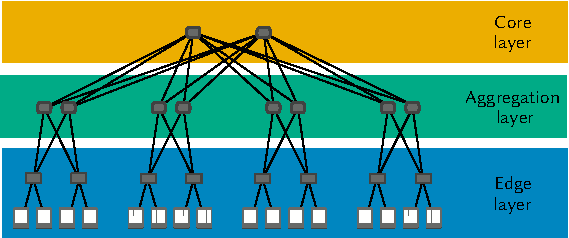
\includegraphics{cloud/data_centers/problem_formulation/figures/architecture}
  \caption{Three-tier data center architecture}
  \label{fig:sec:cloud:data_centers:problem_formulation:3-tier_datacenter}
\end{figure}


We assume, that new jobs entering the system arrive with exponentially distributed inter-arrival time.
When a job in form of a packet arrives at the \gls{POD}, it is forwarded to an idle server.
If no idle server is available, the job is queued.
Once a server finishes processing its current job, it picks another one from the queue.

Our goal is now to evaluate how much power is consumed in a data center and how much can be saved when servers, not processing any job, are switched off.
Therefore, we developed two different data center models.
The first model, the \emph{default data center}, consists of two-state servers only which are either \emph{busy} or \emph{idle}, as shown in \reffig{fig:sec:cloud:data_centers:problem_formulation:servers:idle_busy}) 
For the second model, a more \emph{energy-efficient data center}, a subset of the servers may additionally be switched on and \emph{off} on demand, shown in \reffig{fig:sec:cloud:data_centers:problem_formulation:servers:idle_busy_off} as recommended in~\cite{EPA2007}.

\begin{figure}
	\begin{subfigure}[b]{\textwidth}
	\centering
	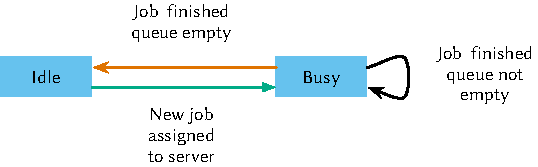
\includegraphics{cloud/data_centers/problem_formulation/figures/idle_busy}
	\caption{2-state server model}\label{fig:sec:cloud:data_centers:problem_formulation:servers:idle_busy}
	\end{subfigure} 
	\begin{subfigure}[b]{\textwidth}
	\centering
	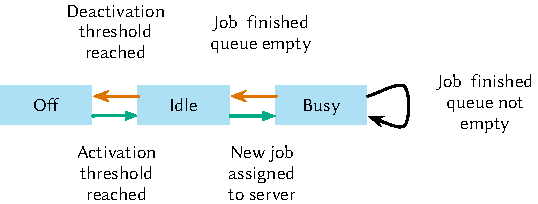
\includegraphics{cloud/data_centers/problem_formulation/figures/idle_busy_off}
	\caption{3-state model of a reserved server}\label{fig:sec:cloud:data_centers:problem_formulation:idle_busy_off}
	\end{subfigure}

	\caption{CPower state transition on a per server level}\label{fig:sec:cloud:data_centers:problem_formulation:servers}
\end{figure}

\subsection{Default Data Center}\label{sec:cloud:data_centers:problem_formulation:default_data_center}
For the default data center model, each of the \(n\) servers is either on and processing a job or on and idle as depicted in \reffig{fig:sec:cloud:data_centers:problem_formulation:servers:idle_busy}.
If a busy server finishes processing a job and the queue is empty, the server becomes idle. Once a new job is assigned to a yet idle server, the server becomes busy.
According to our measurements of a server with an Intel twelve core processor \SI{2.67}{\giga\hertz} and \SI{32}{\giga\byte} RAM, a server currently processing a job consumes \(e_{\text{busy}} = \SI{240}{\watt}\)
An idle server still consumes \(e_{\text{idle}} = \SI{170}{\watt}\).

\subsection{Energy-Efficient Data Center}\label{sec:probform_3states}
For the second model, we differentiate between two types of servers.
\(n\) base-line servers which are always on and \(m\) reserved servers to be enabled on demand.
If they are enabled, their power consumption is similar to that of the default data center model.
If they are disabled, each server consumes \(e_\text{off} = \SI{0}{\watt}\).
The \(n\) servers which are always enabled consume the same power as in the default data center model.
If the system queue has a length exceeding \(\theta_2\) where \(\theta_2 \in (0, m)\) holds, the \(m\) reserved servers are enabled and stay enabled until the total number of jobs in the system drops to \(\theta_1\) for \(\theta_1 \in (0, n)\).
The transition between power levels for each of the reserved servers is depicted in \reffig{fig:sec:cloud:data_centers:problem_formulation:idle_busy_off}.

The energy-efficient data center operation model with the parameters \(\theta_1\) and \(\theta_2\) is depicted in \reffig{fig:sec:cloud:data_centers:problem_formulation:model} and described in detail in the next section.

\begin{figure}
  \centering
  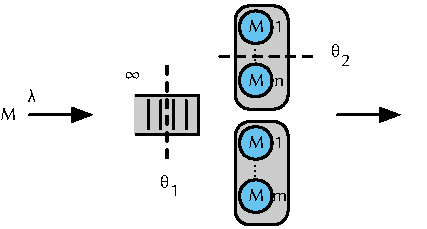
\includegraphics{cloud/data_centers/problem_formulation/figures/model}
  \caption{System model for an energy-efficient operation}
  \label{fig:sec:cloud:data_centers:problem_formulation:model}
\end{figure}
\subsection{Modeling}\label{sec:cloud:data_centers:modeling}
In this section, we first discuss the default data center model, where a server can either be idle or busy, processing a job. Afterwards, the energy-efficient data center model with the three states is set up.

\subsubsection*{Default Data Center}\label{sec:cloud:data_centers:modeling:default}
We consider new jobs arriving at a \gls{POD} with exponential \gls{IID} inter-arrival times with rate \(\lambda\) and each server accepts only one job at a time with an exponentially distributed service time with mean \(\frac{1}{\mu}\).
Then, the system can be modeled using a simple \(M/M/n\) delay system.
Here, the random variable \(X\) gives the number of jobs in the system and \(x(i)\) is the stationary probability that \(i\) jobs are currently in the system.

\subsubsection*{Energy Efficient Data Center}\label{sec:cloud:data_centers:modeling:energy_efficient}
\subsection{Analysis of Proposed Data Centre Models}\label{sec:cloud:data_centers:closed_form_solution}
Using the macro state equations discussed in \refsec{sec:cloud:data_centers:modeling}, there are multiple ways to obtain the state probabilities.
This section examines the different approaches.

\subsubsection*{System of Linear Equations}
First, it is possible to directly solve the system of linear equations implied by the micro or macro states.
Solvers for linear equation systems scale cubic in the dimension of the matrix, which in this case is bounded by the system size.
Especially for a large numbers of server, this prevents an exhaustive search of the parameter space.

\subsubsection*{Closed-form Solutions}
Thus, we obtain closed form solutions for the state probabilities.
These equations can be derived by recursively applying the macro state equations.

All equations feature a factor \(x(0, 0)\) which in turn can be calculated using the normalisation property given in \refeq{eq:cloud:data_centers:modeling:normative}.
Due to the length of the individual formulas, the following shorthand is introduced:
For each state probability \(x(i, j)\) depending on the factor \(x(0,0)\) we define \(\bar{x}(i, j) = x(i, j) \cdot x(0, 0)^{-1}\), i.e. we cancel the factor.

For \(0 < i <\theta_1\), we get
\begin{align*}
x(i, 0) &= x(0, 0) \cdot \frac{a^i}{i!}.
\end{align*}
As a further shorthand for substitution, we define
\begin{align*}
s_i&=\sum_{k=0}^{i}a^k(n-k-1)!.
\end{align*}
Using this definition, we get the state probability for \(\theta_1\) jobs in the system with activated reserved servers as
\begin{align*}
x(\theta_1, 1) &= x(0, 0)\cdot \frac{a^{n+\theta_2+1}}{\left(1+\frac{a}{\theta_1}\right)}
\cdot\frac{\left(\theta_1-1\right)!\left(\frac{(1-a^{\theta_2})\theta_1}{1-a}+a^{\theta_2}s_{n-\theta_1}\right)}{n^{\theta_2}n!\left(n-\theta_1+1\right)!}.
\end{align*}
For \(\theta_1\leq i\leq n\), we get
\begin{align*}
x(i, 0) = x(0, 0) &\cdot \left(\frac{\bar{x}(n, 0) a^{i-\theta_1+1}}{(i-\theta_1+1)!} - \frac{\bar{x}(\theta_1,1) \theta_1 s_{i-\theta_1}}{i!}\right).
\end{align*}
And for \(n<i\leq n+\theta_2\), we get
%TODO single line
\begin{align*}
x(i, 0) = x(0, 0) &\cdot \left(\frac{\bar{x}(n,0) a^{i-\theta_1+1}}{n^{i-n}(n-\theta_1+1)!}\right.\\
&\left.-\bar{x}(\theta_1,1)\left(\frac{\theta_1 s_{n-\theta_1} a^{i-n}}{n!} + \frac{\theta_1(1-a^{i-n})}{1-a}\right)\right).
\end{align*}

Thus, we have all probabilities for system states where only the baseline servers are active. For the reserved servers, we obtain state probabilities for \(\theta_1<i\leq n+\theta_2+1\) as
\begin{align*}
x(i, 1) = x(0, 0) \cdot \left(\bar{x}(\theta_1, 1)\frac{a^{i-\theta_1}\theta_1!}{i!} + \bar{x}(n+\theta_2,0)\sum_{k=1}^{i-\theta_1}\frac{a^k(i-k)!}{i!}\right).
\end{align*}

For \(n+\theta_2+1 < i \leq n + m\), we get
\begin{align*}
x(i, 1) = x(0, 0)\cdot \bar{x}(n+\theta_2+1,1) \cdot\frac{a^{i-(n+\theta_2+1)}(n+\theta_2+1)!}{i!},
\end{align*}
and finally for \(i>n+m\)
\begin{align*}
x(i, 1) = x(0, 0)\cdot \bar{x}(n+m,1) \left(\frac{a}{n+m}\right)^{i-(n+m)}.
\end{align*}
As discussed earlier, the probability of an empty system is given by the normalisation condition:
\begin{align*}
x(0, 0)=\left(1 +\sum_{k=1}^{n+\theta_2}\bar{x}(k, 0) + \sum_{k=\theta_1}^{\infty}\bar{x}(k,1)\right)^{-1}.
\end{align*}

While these closed form solutions allow for the derivation of analytical properties of the model, performing a numerical analysis of a given parameter space is difficult due to numerical instability of the equations.

\subsubsection*{Recursive Algorithm}
To avoid these problems, we introduce a recursive algorithm to calculate the state probabilities based on the macro state equations.
To this end, our we first define \(x(0,0)\) as a constant \(K_0\), and then iteratively computes the state probabilities.
For an earlier application of this concept, see \cite{Trangia1997}.
First, we calculate \(x(i,0)\) for \(0<i<\theta_1\) as a factor of \(x(0,0)\) using \refeq{eq:cloud:data_centers:modeling:energy_efficient:S1_1}.
To obtain the probability for \(x(\theta_1,0)\), not only \(x(\theta_1 -1, 0)\), but \(x(\theta_1, 1)\) is required, which we have not obtained yet.
As this is the case with all \(x(i,0)\) for \(\theta_1 \leq i \leq n + \theta_2\) we implicitly introduce a second constant \(K_1\) for \(x(\theta_1, 1)\) and calculate all \(x(i,0)\) for \(\theta_1 \leq i \leq n + \theta_2\) as a linear combination of \(x(\theta_1 - 1,0)\) and \(K_1\) as follows:
\begin{equation}
x(i, 0) = x(\theta_1 - 1, 0) u_i + K_1 v_i.\label{eq:cloud:data_centers:modeling:closed_form_solution:linear_combination}
\end{equation}
For \(i = \theta_1\), \refeq{eq:cloud:data_centers:modeling:energy_efficient:S1_2} requires \(u_{\theta_1} = \frac{a}{\theta_1}\) and \(v_{\theta_1} = 1\).
Continuing this pattern by successively applying \refeq{eq:cloud:data_centers:modeling:energy_efficient:S1_2} for \(\theta_1 < i \leq n\), we get
\begin{align*}
u_i &= \frac{a}{i}u_{i-1},\\
v_i &= \frac{a}{i}v_{i-1} + \frac{\theta_1}{i}.
\end{align*}
We use \refeq{eq:cloud:data_centers:modeling:energy_efficient:S1_3} to continue for \(n < i \leq n + \theta_2\), and get
\begin{align*}
u_i &= \frac{a}{n}u_{i-1},\\
v_i &= \frac{a}{n}v_{i-1} + \frac{\theta_1}{n}.
\end{align*}
Thus, we arrive at a probability for \(x(n + \theta_2,0)\) depending on \(x(\theta_1 -1,0)\), which we have obtained, and \(K_1 = x(\theta_1,1)\) which we still need to acquire:
\begin{equation*}
x(n+\theta_2,0) = x(\theta_1 -1,0) u_{n+\theta_2} - K_1 v_{n+\theta_2}.
\end{equation*}
We apply \refeq{eq:cloud:data_centers:modeling:energy_efficient:S3} and solve for \(K_1\) and obtain
\begin{equation*}
K_1 =  \frac{\frac{a}{\theta_1} u_{n+\theta_2}}{\frac{a}{\theta_1} v_{n + \theta_2} + \theta_1} x(\theta_1 - 1, 0),
\end{equation*}
which allows to calculate the probabilities of \(x(i,0)\) for \(\theta_1 \leq i \leq n + \theta_2\) using \refeq{eq:cloud:data_centers:modeling:closed_form_solution:linear_combination}.

We can now obtain the probabilities for states in which the reserved servers have been activated, beginning with \((\theta_1 + 1,1)\) we apply \refeq{eq:cloud:data_centers:modeling:energy_efficient:S2_1} for all \(\theta_1 < i \leq n + \theta_2 + 1\) and get
\begin{equation*}
x(i,1) = \frac{a}{i}(x(i-1,1)+ x(n+\theta_2,0))
\end{equation*}
which we can calculate directly as all probabilities are known in relation to \(K_0\).
We continue applying \refeq{eq:cloud:data_centers:modeling:energy_efficient:S2_2} and obtain
\begin{equation}
x(i,1) = \frac{a}{i}(x(i-1,1) + x(n+\theta_2,0))\label{eq:cloud:data_centers:modeling:energy_efficient:probability_greater_nm}
\end{equation}
for \(n + \theta_2 + 1 < i \leq n + m\).

Finally, we need to calculate the probability that the system is in states \((i,1)\) for \(i > n + m\) where we need to obtain
\begin{equation*}
x(i>n+m,1) = \sum_{i = n + m + 1}^{+ \infty} x(i,1).
\end{equation*}
Due to the recursive definition of \refeq{eq:cloud:data_centers:modeling:energy_efficient:S2_3}, we can write
\begin{equation*}
x(i,1) = \rho x(i-1,1) = x(n + m,1)\rho^{i-(n+m)}
\end{equation*}
for \(\rho = \frac{a}{n + m}\) and \(i > n + m\).

Applying this redefinition to \refeq{eq:cloud:data_centers:modeling:energy_efficient:probability_greater_nm} we get
\begin{align*}
x(i>n+m,1) &= \sum_{i = n + m + 1}^{+ \infty} x(i, 1)\\
&= x(n+m,1)\sum_{i=1}^{+\infty} \rho^i.\nonumber
\end{align*}
After applying the properties of the geometric series and basic transformations we get
\begin{equation*}
x(i>n+m,1) =x(n + m,1) \frac{2-\rho}{1-\rho}.
\end{equation*}
Now that all probabilities are known in relation to \(K_0\), we apply \refeq{eq:cloud:data_centers:modeling:normative} to obtain the inverse of \(K_1\) and norm our values to obtain the real probabilities.

This approach allows for a fast and numerically stable calculation of the state probabilities and can be used to compute the required performance metrics for the complete parameter space.

\subsection{Inferring State Transitions and Deriving Metrics}\label{sec:network:network_traces:performance_evaluation}
A \gls{UE}’s firmware triggers \gls{RRC} state transitions based on application traffic.
While solutions exist to capture RRC state transitions on specific hardware~\cite{zayas2010} they are not available for all modern smartphone platforms.
Other options to measure the required information include using costly hardware and use specific \glspl{UE}, usually not available to researchers and application developers.
This prevents the developers from evaluating the effect of their applications on the overall health
of the network.
Consequently, they can not take measures to prevent the harmful behaviour of their applications.
However, it is possible to infer the \gls{RRC} state transitions for a given packet trace if the network configuration is known.

First, we describe the setup used to capture network packet traces for arbitrary apps.
Then, we give an algorithm to infer the \gls{RRC} state transitions for a given packet trace.
Based on these state transitions, we can calculate the number of signalling messages generated
by the packet trace. 
Finally, we use the information on when which \gls{RRC} state was entered to calculate the power drain of the \gls{UE}’s radio interface.

\subsubsection*{Measurement Procedure and Setup}\label{sec:network:network_traces:performance_evaluation:measurement}
To investigate the behaviour of the application under study, we capture traffic during a typical use of the application on a \emph{Samsung Galaxy SII} smartphone.
The smartphone runs the Android operating system and is connected to the \gls{3G} network of a major German network operator.
To obtain the network packet traces we use the \texttt{tcpdump} application.
This application requires \emph{root} privileges which are obtained by rooting the device and installing the custom \emph{cyanogenmod} ROM \footnote{\url{http://www.cyanogenmod.org}, Accessed: November, \(21^{st}\) 2015}.
Once \texttt{tcpdump} is installed and running, we start the application under study and capture packet traces while the application is running.
Then, the \emph{android debugging bridge} is used to copy the traces to a workstation.
The traces contain \gls{IP} packets embedded in Linux Cooked Captures.
We require the \gls{IP} packets, thus we extracted the \gls{IP} packets which are used during the analysis to follow.

\subsubsection*{Inferring Network State}\label{sec:network:network_traces:performance_evaluation:inferring_network_state}
In this section we study the influence of the application traffic on \gls{RRC} state transitions and signalling messages.
Since \gls{RRC} state transitions can not be captured using commonly available tools, we introduce an algorithm to infer \gls{RRC} state transitions from \gls{IP} packet traces.
Using this algorithm we analyse the \gls{RRC} state transition frequency and signalling message load for the Two State Model and Three State Model.

Traffic below the network layer can not be measured without specific equipment which interfaces with the proprietary firmware of the \gls{UE} and is often out of reach for developers interested in assessing the impact of their applications on the network.
Based on the Two State and Three State models introduced in \refsec{sec:network:background:umts_rrc}, we process \texttt{tcpdump} captures of the application traffic.
However, it should be noted that this method is not restricted to a specific network model, but can be extended to any other network model as well.
Using these captures, we extract the timestamps when \gls{IP} packets are sent or received.
Furthermore, we require the timer values of the transition from \gls{RRC_DCH} state to \gls{RRC_FACH} state, \gls{TDCH}, and the timer for the transition between \gls{RRC_FACH} and \gls{RRC_idle} states, \gls{TFACH}.
Based on these informations \refalg{alg:network:network_traces:performance_evaluation:inferring_network_state:inference_algorithm} infers the timestamps of state transitions according to the \gls{3GPP} specification \cite{3GPP_RRC_Spec} for the Three State Model.
This algorithm can be simplified to also work for the Two State Model. 
Alternatively, a method to post process the results of the algorithm to obtain results for the Two State Model is given at the end of this section.
The algorithm first computes the inter-arrival times of all packets.
Then, each timestamp is considered.
If the \gls{UE} is currently in \gls{RRC_idle} state, a state transition to \gls{RRC_DCH} occurs at the moment the packet is sent or received.
If the inter-arrival time exceeds the \gls{TDCH} timer the \gls{UE} transitions to \gls{RRC_FACH} \gls{TDCH} seconds after the packet was sent or received.
Similarly, if the inter-arrival time exceeds both the \gls{TDCH} and \gls{TFACH} timers a state transition to \gls{RRC_idle} occurs \gls{TDCH} seconds after the state transition to \gls{RRC_FACH}.

\begin{algorithm}
  \begin{algorithmic}
    \Require{Packet arrival timestamps \emph{ts}\\
    \gls{RRC_DCH} to \gls{RRC_FACH} timer \gls{TDCH}\\
    \gls{RRC_FACH} to \gls{RRC_idle} timer \gls{TFACH}}
    \Ensure{Times of state transition \emph{state\_time}\\
    New states after state transitions \emph{state}}
    \State \texttt{interarrival(i)} $\leftarrow$ \emph{ts}(i+1) - \emph{ts}(i)
    \State \texttt{index} $\leftarrow 0$
    \ForAll{ts(i)}
      \If{\texttt{state(index)} = \gls{RRC_idle}}
        \State \texttt{index} $\leftarrow$ \texttt{index} + 1
        \State \texttt{state(index)} $\leftarrow$ \gls{RRC_DCH}
        \State \texttt{state\_time(index)} $\leftarrow$ ts(i)
      \EndIf
      \If{\texttt{interarrival}(i-1) $> \gls{TDCH}$}
        \State \texttt{index} $\leftarrow$ \texttt{index} + 1
        \State \texttt{state(index)} $\leftarrow$ \gls{RRC_FACH}
        \State \texttt{state\_time(index)} $\leftarrow$ ts(i) $+ \gls{TDCH}$
      \EndIf
      \If{\texttt{interarrival}(i-1) $> \gls{TDCH} + \gls{TFACH}$}
        \State \texttt{index} $\leftarrow$ \texttt{index} + 1
        \State \texttt{state(index)} $\leftarrow$ \gls{RRC_idle}
        \State \texttt{state\_time(index)} $\leftarrow$ ts(i) $+ \gls{TDCH} + \gls{TFACH}$
      \EndIf
    \EndFor
  \end{algorithmic}
  \caption{Inferring \headershortacr{RRC} state transitions based on \headershortacr{IP} timestamps.}
  \label{alg:network:network_traces:performance_evaluation:inferring_network_state:inference_algorithm}
\end{algorithm}

Decreasing power drain of their devices is always a goal of \gls{UE} vendors.
A straightforward way to achieve this, if only the wellbeing of the \gls{UE} is considered, is to transition from \gls{RRC_DCH} state to \gls{RRC_idle} as soon as no additional data is ready for sending.
While this transition is not directly available in the 3GPP specification for the \gls{RRC} protocol \cite{3GPP_RRC_Spec}, a \gls{UE} may reset the connection, effectively transitioning from any state to \gls{RRC_idle}.
This behaviour can be modeled using the Two State Model introduced in \refsec{sec:network:background:umts_rrc}.

State transitions for the Two State Model can be calculated using a similar algorithm.
Alternatively, the behaviour of the Two State Model can be emulated using \refalg{alg:network:network_traces:performance_evaluation:inferring_network_state:inference_algorithm} if \gls{TFACH} is set to \SI{0}{\second} and all state transitions to \gls{RRC_FACH} are removed in a post processing step.

\subsubsection*{Calculating Signalling Frequency and Power Drain}\label{sec:network:network_traces:calculating_metrics}

\begin{table}
\centering
  \caption{Number of signalling messages per \headershortacr{RRC} state transition perceived at the \headershortacr{RNC} \cite{3GPP_RRC_Spec}.}
  \label{tab:network:network_traces:calculating_metrics:signalling_messages}
\begin{tabular}{lccc}
	\toprule
    from/to & \gls{RRC_idle} & \gls{RRC_FACH} & \gls{RRC_DCH}\\
    \midrule
    \gls{RRC_idle} & -- & 28 & 32\\
    \gls{RRC_FACH} & 22 & -- & 6\\
    \gls{RRC_DCH} & 25 & 5 & --\\
    \bottomrule    
	\end{tabular}
\end{table}

In reality, the number of state transitions is not the metric of most importance if network signalling is to be evaluated.
Each state transition results in a number of \gls{RRC} messages between the \gls{UE} and different network components.
For this study we consider the number of messages observed at the \gls{RNC}, which can be found in \cite{3GPP_RRC_Spec} and is summarized in \reftab{tab:network:network_traces:calculating_metrics:signalling_messages}.
It can be seen that transitions from or to the \gls{RRC_idle} state are especially expensive in terms of number of messages sent or received.
This is due to the fact that upon entering or leaving the \gls{RRC_idle} state, authentication has to be performed. 
Note that for the Two State Model only transitions from or to the \gls{RRC_idle} state occur.
This results in the fact that for the same network packet trace the number of signalling messages occurring in the Two State Model is generally higher than in the Three State Model.
To obtain the total number of signalling messages, we weight the number of state transitions with the number of messages sent per state transitions.
Then, we average the number of state transitions over the measurement duration to obtain a metric for the signalling load at the \gls{RNC}, i.e. the \gls{SF}.
The inference algorithm does not differentiate between state changes caused by upstream or downstream traffic.
State changes caused by downstream traffic usually generate some additional signalling messages, as paging is involved.
The inference algorithm can easily be enhanced to support this behaviour.
However, the results discussed in the next section would only change quantitatively.
Furthermore, the algorithm can be adapted to new networking models or other numbers of signalling messages sent per state transition.

\begin{table}
  \centering
  \caption{Power consumption of the \headershortacr{UE} radio interface depending on current \headershortacr{RRC} state \cite{Qian2011a}.}
  \label{tab:network:network_traces:calculating_metrics:power_consumption}  
  \begin{tabular}{lc}
  	\toprule
    \gls{RRC} State & Power Consumption\\
    \midrule
    \gls{RRC_idle} & \SI{0}{\milli\watt}\\
    \gls{RRC_FACH} & \SI{650}{\milli\watt}\\
    \gls{RRC_DCH} & \SI{800}{\milli\watt}\\
    \bottomrule
  \end{tabular}
\end{table}

From a users point of view, the signalling message frequency is of little importantance.
The user is interested in a low power drain as this increases the battery life of the device.
To calculate the battery life, we use the time when state transitions occurred, and the information about the state the transition was to, to calculate the relative amount of time that was spent in each state.
Given the relative time spent in each state, we use \reftab{tab:network:network_traces:calculating_metrics:power_consumption}, taken from \cite{Qian2011a}, to compute the \gls{PD} of the radio interface during the measurement phase.
We focus on the power drain of the radio interface, as it is possible to measure the aggregated power drain using out of the box instrumentation techniques provided by the hardware vendor.